\documentclass[[10pt,journal]{IEEEtran}
\usepackage{blindtext}
\usepackage{graphicx}
\usepackage{cmap}	
\usepackage{lmodern}
\usepackage{booktabs, multicol, multirow}
\usepackage{graphicx,url}
\usepackage[T1]{fontenc}
\usepackage[utf8]{inputenc}
\usepackage{float}
\usepackage{fixltx2e}
\usepackage{amsfonts}
\usepackage{amsmath}
\newcommand{\textoverline}[1]{$\overline{\mbox{#1}}$}

\usepackage{anyfontsize}

\hyphenation{op-tical net-works semi-conduc-tor}


\begin{document}
\title{Um estudo da interferência entre máquinas virtuais em seus desempenhos \\~\\
\textit{A Study on interference among virtual machines into their performances}}

%\author{
%\begin{tabular}[t]{cc} 
%\fontsize{11}{12}\textbf{Maxwell Santos, Paulo Meirelles} & \textbf{Rafael Manzo} \\
%                        Faculdade UnB Gama        & Instituto de Matemática e Estatística  \\ 
%                        Universidade de Brasília  & Universidade de São Paulo\\
%                        Brasília, Brasil          & São Paulo, Brasil \\
%                        llewxam150@gmail.com, paulormm@unb.br  & rr.manzo@gmail.com\\
%\end{tabular}
%}

\maketitle

%------------------------------------------------------------------------------
\begin{resumo}
Com o recente crescimento da computação em nuvem, tornaram-se recorrentes
questionamentos feitos com relação a perda de desempenho em ambientes
virutalizados. Neste contexto, realizamos uma série de coleta de dados,
desenvolvemos procedimentos e selecionamos um conjunto de ferramentas
tipicamente utilizadas para medição de desempenho em sistemas computacionais.
Nossos resultados mostram que o grau de interferência é variável de acordo com
o tipo de aplicação que está sendo executada nas máquinas virtuais, e que é
possível aplicar modelos estatísticos para predição de desempenho de uma
aplicação.
\end{resumo}

\begin{abstract}
Cloud computing is growing and there are recurrent questions about performance
loss in virtualized environments. In this context, we have performed several
data collection, developed procedures and selected a set of tools typically
used to measure performance in computational systems. Our results show that the
interference degree is variable according to the type of application that is
running in the virtual machines. In addition, it is possible to apply
statistical models for performance prediction of an application.
\end{abstract}

\begin{IEEEkeywords}
Cloud Computing, Virtualization, Performance Systems.
\end{IEEEkeywords}

\section{Introdução}
\label{sec:introducao}

Devido as tendências como computação em nuvem, TI verde e a consolidação de
servidores, a virtualização vem ganhando cada vez mais importância.
Anteriormente usada para o uso mais eficiente de recursos físicos de
\textit{mainframes}, hoje em dia, a virtualização é novamente utilizada para
executar múltiplas máquinas virtuais em uma infraestrutura compartilhada,
aumentando dessa forma a utilização de recursos, promovendo flexibilidade e
centralizando a administração \cite{huber2011}. Essa popularidade deve-se
também ao amplo uso de infraestruturas distribuídas por parte de sistemas
computacionais modernos, o que colabora para o desenvolvimento de aplicações
colaborativas e promove o compartilhamento de recursos remotos
\cite{popiolek2012}.

Neste contexto, a computação em nuvem, alinhada à virtualização, permite um
conjunto de servidores físicos disponibilizar dezenas ou centenas de máquinas
virtuais. Desse modo, proporciona-se aumento na escalabilidade, maximizando o
uso de recursos \cite{popiolek2012}. Entretanto, antes de migrar aplicações de
ambientes não virtuais para ambientes virtuais, é necessário entender como será
o desempenho dessas aplicações nesse novo ambiente \cite{benevuto2006}. A
adoção de servidores virtualizados vem com o aumento de custo na complexidade e
dinâmica do sistema. O aumento da dinâmica é causada pela falta de controle
direto sob o hardware, pelas interações complexas entre as aplicações e cargas
de trabalho que compartilham os mesmos recursos físicos. Em suma, o aumento da
complexidade é causada pela introdução de recursos virtuais que por sua vez
causa uma diferença entre a alocação de recursos físicos e lógicos
\cite{huber2011}.

De acordo com Koh \cite{koh2007}, observa-se que as tecnologias atuais que
possibilitam a criação de máquinas virtuais não fornecem um isolamento efetivo.
Enquanto o \textit{hypervisor} (software responsável pela disponibilização e
gerenciamento de máquinas virtuais) reparte os recursos e os aloca para as VMs,
o comportamento de cada VM ainda pode afetar o desempenho das outras de maneira
negativa devido ao uso de recursos compartilhados no sistema.

Nesse contexto, entende-se que é fundamental compreender os fatores que
impactam no desempenho de ambientes virtualizados, bem como quantificar e
avaliar o desempenho de aplicações em tais ambientes para que possa
implantá-las e configurá-las adequadamente. Tendo isso em vista, torna-se
importante o conhecimento de ferramentas e técnicas ou metodologias que
auxiliem nas atividades relacionadas à análise de desempenho em ambientes
virtualizados.

Assim, neste trabalho foi realizado um estudo de interferência de desempenho em
ambientes virtuais ocasionado por um conjunto de aplicações. Através das
métricas de desempenho de sistema foi possível observar que determinadas
aplicações, dado seu perfil de execução, ocasionam maior grau de interferência
do que outras quando executadas em máquinas virtuais que compartilham o mesmo
servidor. Além disso, a partir dos dados coletados, foi possível aplicar
mecanismos de predição de desempenho em função da carga de trabalho que está
sendo aplicada. Esses mecanismos de predição foram desenvolvidos por Koh
\cite{koh2007}. Adicionalmente, neste trabalho aplica-se uma análise de
regressão polinomial baseada nestes mecanismos. Um comparativo entre esses
mecanismos foi realizado, sendo possível discutir que a análise de regressão
polinomial foi capaz de predizer o desempenho com taxas de erros menores do que
os mecanismos apresentados no trabalho por Koh \cite{koh2007}.  


\section{Cálculo da Interferência}
\label{sec:calculo-interferencia}

Para o estudo proposto por este trabalho foi definido um  ambiente de testes
que consiste no uso de máquinas virtuais com aplicações voltadas para
realização de testes de \textit{benchmark}. Tais aplicações foram definidas a
partir do trabalho de Koh \cite{koh2007}, tendo essas sido escolhidas visando o
estresse de vários aspectos de sistema e de \textit{hardware}. A fim de se ter
comodidade na criação e destruição dessas máquinas virtuais foi utilizado o
OpenNebula como ferramenta de computação em nuvem e como \textit{hypervisor}
foi utilizado o \textit{kvm}. As máquinas virtuais possuíam, como configuração,
sistema operacional \textit{Centos 7}, espaço em disco de 15GB e 1GB de memória
\textit{RAM}. Em um primeiro momento as aplicações foram instaladas e testadas
de modo que se pudesse observar quais são os comandos utilizados para
funcionamento das mesmas, em seguida foram criados \textit{snapshots} das
máquinas virtuais com o auxílio provido pelo \textit{OpenNebula}.

Entre as aplicações escolhidas estão típicas provedoras de \textit{stress}
computacional no cotidiano, tais como compilação de código fonte, compressão e
encriptação de arquivos e processamento de imagens, bem como, ferramentas
voltadas para geração de testes de \textit{benchmark} tais como
\textit{Cachebench} e \textit{AIM Benchmark suite}. São elas: Add\_double,
Bzip2, Gzip, Ccrypt, Cachebench, Cat, Grep, cp, dd, Iozone, Make e Povray.

%Add\_double (\url{sourceforge.net/projects/aimbench}), Bzip2 (\url{bzip.org}),
%Gzip (\url{gzip.org}), Ccrypt (\url{ccrypt.sourceforge.net}), Cachebench
%(\url{icl.cs.utk.edu/projects/llcbench/cachebench.html}), Cat
%(\url{linux.die.net/man/1/cat}), Grep (\url{linux.die.net/man/1/grep}), Dp
%(\url{linux.die.net/man/1/cp}), DD (\url{linux.die.net/man/1/dd}), Iozone
%(\url{iozone.org}), Make (\url{linux.die.net/man/1/make}) e Povray
%(\url{povray.org}).

Os procedimentos adotados para o cálculo da interferência seguem os propostos
no trabalho de Koh \cite{koh2007}. Desse modo, duas máquinas virtuais são
criadas em um servidor utilizando \textit{hypervisor} \textit{KVM}. Cada
máquina virtual, denominadas \textit{'dom1'} e \textit{'dom2'} respectivamente,
executa uma das aplicações de \textit{benchmarking}. 

Uma aplicação executando em \textit{dom1} é chamada de aplicação
\textit{foreground}, e a que estiver executando em \textit{dom2} é a aplicação
\textit{background}. Por questões de notação uma aplicação \textit{foreground}
executando contra uma aplicação \textit{background} é denotada como F@B. Um dos
procedimentos adotados é garantir que a aplicação \textit{background} mantenha
sua execução até que a aplicação \textit{foreground} termine. Para o segundo e
terceiro experimento cada aplicação é executada de modo que seja tanto
\textit{background} quanto \textit{foreground}, sendo construída dessa forma
uma matriz \textit{n x n} com todos os possíveis resultados.

A fim de observar o quanto o desempenho é afetado pela interferência gerada por
uma aplicação executada em outra máquina virtual, é feita a medida da
degradação a partir do desempenho padrão de uma aplicação, essa medida
denomina-se pontuação normalizada. Assim, para calcular a pontuação normalizada
de uma aplicação, primeiro é definida a pontuação de desempenho inativa que é a
pontuação de uma aplicação quando executada contra uma máquina virtual inativa,
ou seja, sem nenhuma aplicação executando. Então, em seguida é feito o cálculo
da pontuação normalizada de uma aplicação F contra B, dividindo a pontuação de
desempenho de F contra B pela pontuação de desempenho inativa de F. Assim
define-se NS(F@B), como sendo a pontuação normalizada de F contra B, sendo
PD(F@B) a pontuação de desempenho de uma aplicação F contra uma aplicação B:

\begin{equation}
\label{eq:degradation}
NS(F@B) = PD(F@B)/PD(F@Inativo)
\end{equation}

A partir disso, é feito cálculo do desempenho combinado de duas aplicações, F e
B, em cada máquina virtual:

\begin{equation}
\label{eq:combined}
NS ( F + B ) = NS ( F @ B ) + NS ( B @ F )
\end{equation}


\begin{table}[!htb]
\centering
\caption{Aplicações utilizadas para geração de cargas e trabalho.}
\label{table-aplications}
\resizebox{0.45\textwidth}{!}{
\begin{tabular}{|l|c|c|}
\hline
Nome        & \multicolumn{1}{l|}{Maior Recurso Utilizado} & \multicolumn{1}{l|}{Medida de Desempenho} \\ \hline
Add\_double & CPU                                          & Pontuação                                  \\ \hline
Bzip2       & Misto                                        & Tempo                                      \\ \hline
Cat         & Disco                                        & Tempo                                      \\ \hline
Cachebench  & Memória                                      & Pontuação                                  \\ \hline
Ccrypt      & Misto                                        & Tempo                                      \\ \hline
Cp          & Disco                                        & Tempo                                      \\ \hline
Dd          & Disco                                        & Tempo                                      \\ \hline
Grep        & Disco                                        & Tempo                                      \\ \hline
Gzip        & Misto                                        & Tempo                                      \\ \hline
Iozone      & Disco                                        & Pontuação                                  \\ \hline
Make        & Misto                                        & Tempo                                      \\ \hline
Povray      & Misto                                        & Tempo                                      \\ \hline
\end{tabular}}
\end{table}

Sendo NS(F@B) e  NS(B@F) medidos em dois testes separados. Para medida de
desempenho, são utilizadas as pontuações geradas pelas próprias aplicações.
Entretanto, algumas aplicações, aquelas que não são voltadas para
\textit{benchmark}, não geram pontuações explícitas. Para essas aplicações,
fora definido como o inverso do tempo necessário para sua execuação, como
pontuação de desempenho. Na Tabela \ref{table-aplications} é apresentado o
maior recurso utilizado bem como a medida de desempenho utilizada para cada
ferramenta. Dessa forma, uma pontuação normalizada(F@B) próxima ou igual a 1 é
um resultado que indica que o desempenho de uma aplicação \textit{F} contra
\textit{B} sofreu baixa degradação.


\section{Análise de dados}
\label{sec:analise-dados}

No trabalho de Koh \cite{koh2007} são utilizadas métricas de desempenho a nível
de sistema (denominadas \textit{System-level Workload Characteristics}) de
forma a analisar melhor o grau de interferência em diversos aspectos de sistema
na máquina virtual. Segundo Koh \cite{koh2007}, o fato desse tipo de métrica de
desempenho ser independente de qualquer tipo de microarquitetura subjacente
garante que seja possível ser feitas comparações através dos diferentes tipos
de servidores físicos.

Neste trabalho, para o \textit{KVM} chegou-se a ferramentas como o
\textit{iperf-kvm} e \textit{kvm-stat}. Entretanto, as informações apresentadas
por essas ferramentas não eram claras e, para o caso do \textit{kvm-stat}, não
detalhava por máquina virtual e sim para  \textit{hypervisor} inteiro. Mesmo no
\textit{OpenNebula} as informações apresentadas consistiam em uso de espaço em
disco, memória utilizada e quantidade de \textit{CPU} alocado por máquina
virtual, não sendo essas informações relevantes para o estudo proposto. Assim,
a abordagem escolhida foi o uso de uma ferramentas típica para monitoramento de
desempenho: \textit{iostat} para operações de disco e o \textit{mpstat} para
\textit{CPU}. Assim gerando as seguintes métricas coletadas neste trabalho:

\begin{itemize}

\item \textbf{Porcentagem de uso do \textit{CPU}}(\textit{cpuutil}):
Porcentagem de utilização de \textit{CPU} durante a execução de uma aplicação.
É obtida através da aplicação \textit{mpstat}.

\item \textbf{Requisições de escrita e leitura de disco por segundo
}(\textit{writes\_issued, reads\_issued}) e \textbf{Tempo gasto para escrita e
leitura do disco}(\textit{time\_writing, time\_reading}): Quantidade de
requisições no disco e o tempo para operações de escrita e leitura são bons
indicadores de operações de entrada e saída. Esses valores são coletados
utilizando o \textit{iostat}.

\end{itemize}

A análise dos dados obtidos referentes às métricas de desempenho e às
pontuações normalizadas das aplicações foi baseada no uso de técnicas de
análise multivariada com o intuito de predizer o desempenho das aplicações. Em
suma, usamos a média ponderada com o auxílio da análise por componente
principal (PCA), Regressão Linear e Regressão Polinomial. Para realização da
análise por componente principal utilizamos a ferramenta \textit{Scilab} com o
auxílio da biblioteca \textit{FACT}. Já para a análise de regressão linear e
polinomial utilizamos uma ferramenta de análise statística chamada \textit{R}.

De maneira geral, escolhemos uma aplicação ``U'' a partir do conjunto de
aplicações definidos anteriormente. Em seguida, ao utilizar o restante das
aplicações como um conjunto de referência (B1, B2, ..., Bn), foi feita a
predição da pontuação normalizada de ``U'' contra as outras aplicações (i.e,
NS(U@B1), NS(U@B2), ... NS(U@Bn)), das aplicações contra ``U'' (i.e, NS(B1@U),
NS(B2@U), ... NS(Bn@U)) e de ``U'' contra ele mesmo (NS(U@U)). Assim, para cada
técnica aplicada, foi comparado a pontuação predita com a pontuação real
medida. Para avaliação desse comparativo são calculados a média, mediana e o
maior erro da predição obtido, onde o cálculo do erro da predição é feito pela
equação \ref{eq:predict_error}. Esse procedimento foi feito com todas as
aplicações definidas:

\begin{equation}
\label{eq:predict_error}
\textrm{Erro da predição} = \frac{|\textrm{Pontuação real - Pontuação predita}|}{\textrm{Pontuação real}}
\end{equation}

\subsection{Método da Média Ponderada}

O método da média ponderada é baseado na similaridade entre duas aplicações.
Dessa forma, para calcular a similaridade, primeiro é feito o cálculo da
distância dos vetores de métricas de desempenho de duas aplicações. Dada o
número de dimensões desse vetor (5 métricas de desempenho a nível de sistema),
foi aplicada uma análise de componente principal (PCA) de modo que se reduzisse
a dimensionalidade dos dados sem perda significativa.

Assim, embora as \textit{p} variáveis de um vetor de dados sejam necessárias
para reproduzir a total variabilidade de um sistema, frequetemente muito dessa
variabilidade pode ser representada por uma pequena quantidade \textit{k} de
componentes principais. Dessa forma, os \textit{k} componentes principais podem
substituir  as \textit{p} variáveis iniciais, reduzindo o conjunto de dados
necessários para a análise \cite{johnson1988}.

Uma vez que os dados coletados foram convertidos pela análise de componentes
principal, escolhemos os componentes que representam a maior variabilidade
desses dados. Com isso, através dos dados obtidos, selecionamos três
componentes que representam 94\% da variança total (cada componente representa
53,8\%, 24\%, 16,3\% da variança, respectivamente).

Para cálcular a predição da pontuação de U@Bn, adota-se o seguinte procedimento
apresentado no trabalho de Koh \cite{koh2007}. Primeiro, em cima dos dados
transferidos para PCA calculamos a distância euclidiana do ponto desejado,
U@Bn, para todos os resultados de \textit{benchmark} obtidos e então foram
escolhidos os N pontos de dados mais próximos e definidos como um conjunto dos
mais próximos. A similaridade entre o ponto desejado e um ponto dentro do
conjunto dos mais próximos é definida como o inverso da distância. Então, foi
calculado o peso de cada dado no conjunto dos mais próximos proporcional a
similaridade:

\begin{equation}
\label{eq:prediction} 
w_i = s_i / \sum\limits_{i=1}^{N}s_i
\end{equation}

Onde S\textsubscript{i} é a similaridade de uma aplicação i dentro do conjunto
dos mais próximos. Por fim, a predição da pontuação de U@Bn foi calculada com a
seguinte fórmula:

\begin{equation}
\label{eq:simi} 
NS(U@Bn) = \sum\limits_{i=1}^{N}w_i \cdot NS(i)
\end{equation}

\subsection{Análise de Regressão Linear e Polinomial}

Análise de regressão é uma técnica estatística que tem como intuito analisar a
relação entre uma única variável dependente (critério) e várias variáveis
independentes (preditoras), possibilitando assim, apartir dos valores
conhecidos das variáveis independentes X\textsubscript{1}, X\textsubscript{2},
..., X\textsubscript{n} a predição do valor da variável dependente Y
\cite{hair}. Uma forma clássica da análise de regressão é a regressão linear,
que por vez declara que a variável dependente Y é uma função linear das
variáveis independentes. Assim, sua formulação é feita da seguinte maneira
\cite{johnson1988}:

\begin{equation}
\label{eq:linear} 
 \overline{Y} = a_0 + a_1 \cdot X_1 + a_2 \cdot X_2 + ... + a_n \cdot X_n
\end{equation}

Dessa forma, a regressão linear tem como objetivo determinar os coeficientes
a\textsubscript{0}, a\textsubscript{1}, ... , a\textsubscript{n}, utilizando
para isso o método dos mínimos quadrados, de modo a minimizar o erro
|\textoverline{Y} - Y| \cite{koh2007}. Por mais que a regressão linear seja
amplamente utilizada, sua forma clássica pode ainda assim não ser suficiente
para explicar uma boa quantidade de dados, principalmente aqueles que apresenta
um padrão não linear \cite{pantula}. Desse modo, uma outra forma de análise de
regressão é a regressão polinomial que se modela a partir de uma função
polinomial, e tem como proposta desenvolver aproximações para relações
curvilíneas ou não lineares. Os polinômios são transformações de pontência de
uma variável independente que acrescentam uma componente não-linear para cada
pontência adicional da variável independente. A construção de seu modelo
procede da seguinte maneira \cite{hair}:

\begin{equation}
\label{eq:polinomio} 
 \overline{Y} = a_0 + a_1 \cdot X_1 + a_2 \cdot X^2 + a_3 \cdot X^3 + ... + a_n \cdot X^n
\end{equation}

\begin{table}[!htb]
\centering
\caption{Tabela de coeficientes para regressão linear}
\label{tab:coeficiente_linear}
\begin{tabular}{|l|c|}
\hline
\multicolumn{1}{|c|}{X}   & \multicolumn{1}{l|}{Coeficientes} \\ \hline
write\_issued & 3,44                             \\ \hline
read\_issued  & 1,29                             \\ \hline
write\_time   & -1,37                            \\ \hline
read\_time    & -3,91                            \\ \hline
cpu\_util     & 5,15                             \\ \hline
a\textsubscript{0}           & 4,99                             \\ \hline
\end{tabular}
\end{table}

\begin{table}[]
\centering
\caption{Tabela de coeficientes para regressão polinomial}
\label{tab:coeficiente_poli}
\begin{tabular}{|c|c|c|c|}
\hline
\multicolumn{1}{|l|}{Variável} & \multicolumn{1}{l|}{Coeficientes} & \multicolumn{1}{l|}{Variável} & \multicolumn{1}{l|}{Coeficientes} \\ \hline
x\textsubscript{1}                             & -6,26E-03                        & $x\textsubscript{1} \cdot x\textsubscript{4}$                         & 4,27E-05                         \\ \hline
x\textsubscript{1}\textsuperscript{2}                            & 1,26E-05                         & $x\textsubscript{2} \cdot x\textsubscript{4}$                       & -7,23E-05                        \\ \hline
x\textsubscript{2}                             & 1,49E-03                         & $x\textsubscript{3} \cdot x\textsubscript{4}$                                                & -4,00E-05                        \\ \hline
$x\textsubscript{1} \cdot x\textsubscript{2}$                          & 1,60E-05                         & x\textsubscript{4}\textsuperscript{2}                           & 3,13E-05                         \\ \hline
x\textsubscript{2}\textsuperscript{2}                            & 2,42E-06                         & x\textsubscript{5}                            & -1,17E-02                        \\ \hline
x\textsubscript{3}                             & 1,20E-02                         & $x\textsubscript{1} \cdot x\textsubscript{5}$                                                                       & 6,42E-05                         \\ \hline
$x\textsubscript{1} \cdot x\textsubscript{3}$                        & -2,39E-05                        & $x\textsubscript{2} \cdot x\textsubscript{5}$                                                                       & -1,60E-05                        \\ \hline
$x\textsubscript{2} \cdot x\textsubscript{3}$                          & -3,48E-05                        & $x\textsubscript{3} \cdot x\textsubscript{5}$                                                                       & -1,26E-04                        \\ \hline
x\textsubscript{3}\textsuperscript{2}                            & -5,93E-06                        &$ x\textsubscript{4} \cdot x\textsubscript{5}$                                                                       & 1,08E-04                         \\ \hline
x\textsubscript{4}                             & -9,41E-03                        & x\textsubscript{5}\textsuperscript{2}                         & 1,03E-04                         \\ \hline
\end{tabular}
\end{table}

As Tabelas \ref{tab:coeficiente_linear} e \ref{tab:coeficiente_poli} apresentam
os coeficentes encontrados para regressão linear e regresssão polinomial
respectivamente. Vale acrescentar que na análise de regressão um dos mecanismos
utilizadas para verificação da precisão de um modelo preditivo é o coeficiente
de derterminação (R\textsuperscript{2}). Seu valor varia de 0 a 1, indicando,
em termos de porcentagem, o quanto um modelo conseguie explicar os valores
observados. Assim, se o R\textsuperscript{2} é 0,70 isso significa que 70\% dos
dados coletados são explicados pelo modelo preditivo calculado. O cálculo de
R\textsuperscript{2} é motrada na equação \ref{eq:polinomio}:

\begin{equation}
\label{eq:polinomio}  
R^2 = \frac{ \sum\limits_{i=1}^{N}(\hat{y}_i - \overline{y})^2}{\sum\limits_{i=1}^{N}(y_i - \overline{y})^2}
\end{equation} 

onde \textoverline{y} é a média de todas as observações, y\textsubscript{i} é o
valor da observação individual i e \^{y}\textsubscript{i} é o valor previsto da
observação i \cite{hair}.

Neste trabalho aplicamos tanto a análise de regressão linear quanto a análise
de regressão polinomial, definindo como variável dependente a pontuação
normalizada e como variáveis independentes as métricas de desempenho a nível de
sistema. Os dados coletados, com os valores das métricas de desempenho a nível
de sistema e com as pontuações normalizadas, foram utilizados para a
determinação dos coeficientes. Uma vez que os coeficientes foram calculados
utilizando o método dos mínimos quadrados, aplica-se os dados das métricas de
desempenho a nível de sistema na equação com os coeficientes obtidos,
alcançando dessa forma a predição da pontuação normalizada. Por fim, também são
calculados os valores de R\textsuperscript{2}, a fim de verificar qual modelo
apresenta maior aplicabilidade dentro dos dados coletados.


\section{Análise de Resultados}
\label{sec:resultados}

Inicialmente, em nossas análises, via a pontuação normalizada de um conjunto de
aplicações, observamos que, de maneira geral, algumas aplicações tendem a
sofrer e a causar menos interferência do que outras aplicações. É o caso de
\textit{add\_double}, \textit{cachebench}, \textit{make} e \textit{povray}. Não
por acaso, são ferramentas que não possuem perfis de cargas de trabalho
voltados para operações de \textit{entrada/saída} ( \textit{add\_double} possui
perfil voltado para \textit{cpu}, \textit{make} e \textit{povray} possuem
perfil misto mas mais voltado para operações em \textit{cpu} do que de
\textit{entrada/saída} e \textit{cachebench} é mais voltado para operações no
sistema de memória). Assim, observamos também que essas aplicações, por
possuírem um perfil de carga de trabalho voltado mais para \textit{cpu} e
memória (no caso do \textit{cachebench}), praticamente não interferem em
aplicações que possuem um perfil voltado para \textit{operações de
entrada/saída} e nem mesmo sofrem interferência significativa desse tipo de
aplicações.

Por exemplo, observamos que a pontuação de \textit{povray} contra esse conjunto
de aplicações ficou próxima de 1 o que indica o grau de interferência bastante
insignificante, o mesmo ocorrendo com \textit{add\_double}. No caso do
\textit{cachebench}, mesmo tendo sido uma das ferramentas que menos sofreu
interferência, percebemos um grau de interferência mais elevado do que das
outras duas (\textit{povray} e \textit{add\_double}), isso se deve ao fato que
o sistema de memória acaba atuando principalmente em operações de
\textit{cache} tanto em aplicações com perfil voltado para \textit{cpu} quanto
em aplicações com perfil voltado para operações de \textit{entrada/saída}.

Para o restante das aplicações, observamos um grau de interferência maior e com
mais variações dependendo da aplicação que está sendo executada em
\textit{background}. Essas são típicas aplicações de \textit{entrada/saída},
com suas cargas de trabalho atuando em operações de escrita ou leitura em
disco. Por exemplo, observamos que o \textit{dd} e o \textit{cp} são as
aplicações que causam maior degradação no desempenho das aplicações voltadas
para \textit{entrada/saída}. Dessa forma, em uma das combinações realizadas,
executando \textit{Bzip2} contra \textit{dd}, a pontuação ficou abaixo de 0.4,
evidenciando um elevado grau de degradação.

Dada a variação de interferência de desempenho entre essas aplicações,
destacamos que a pontuação alcançada de \textit{gzip} e \textit{bzip2} contra
\textit{grep} indica um grau de degradação de desempenho pequeno ou
praticamente nulo. Em contrapartida, a pontuação alcançada por \textit{cp},
\textit{cat} e \textit{dd} contra \textit{grep} mostra uma degradação do
desempenho maior se comparada com \textit{gzip} e \textit{bzip2} contra
\textit{grep}. Em suma, isso indica que mesmo dentre as aplicações típicas de
\textit{entrada/saída} pode haver um padrão de interferência dado o seu tipo de
execução (escrita ou leitura). 

Posteriormente, aplicamos os mecanismos de predição baseados nos dados
coletados via as métricas de desempenho em nível de sistema e da pontuação
normalizada das aplicações. Com isso, esperamos predizer a pontuação
normalizada de uma aplicação a partir dos valores alcançados nas métricas de
desempenho a nível de sistema. 

\begin{figure}[!htb]
\centering
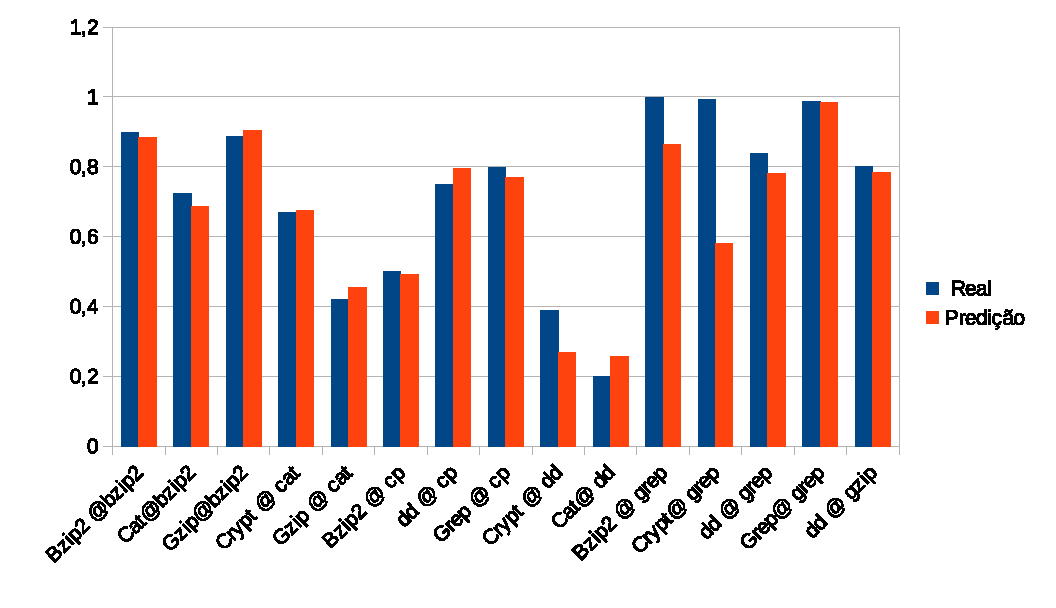
\includegraphics [keepaspectratio=true,scale=0.5]{graficos/mean_predict.eps}
\caption{Comparativo entre a pontuação normalizada real e a pontuação predita utilizando média ponderada com o aúxilio da análise por componente principal.}
\label{mean_predict}
\end{figure}   

A Figura \ref{mean_predict} apresenta um comparativo dos resultados alcançados
utilizando a média ponderada com os valores reais da pontuação normalizada.
Observa-se que no geral de fato o modelo é capaz de predizer com certa
precisão. Observa-se, por exemplo, Bzip2 @ Bzip2 e Crypt @ Cat que os erros de
predição obtidos foram 0,68\% e 0,13\% respectivamente. Entretanto, há alguns
casos que há uma discrepância relevante como por exemplo Crypt @ Grep ao qual o
erro de predição foi de 41,5\%.
   

\begin{figure}[!htb]
\centering
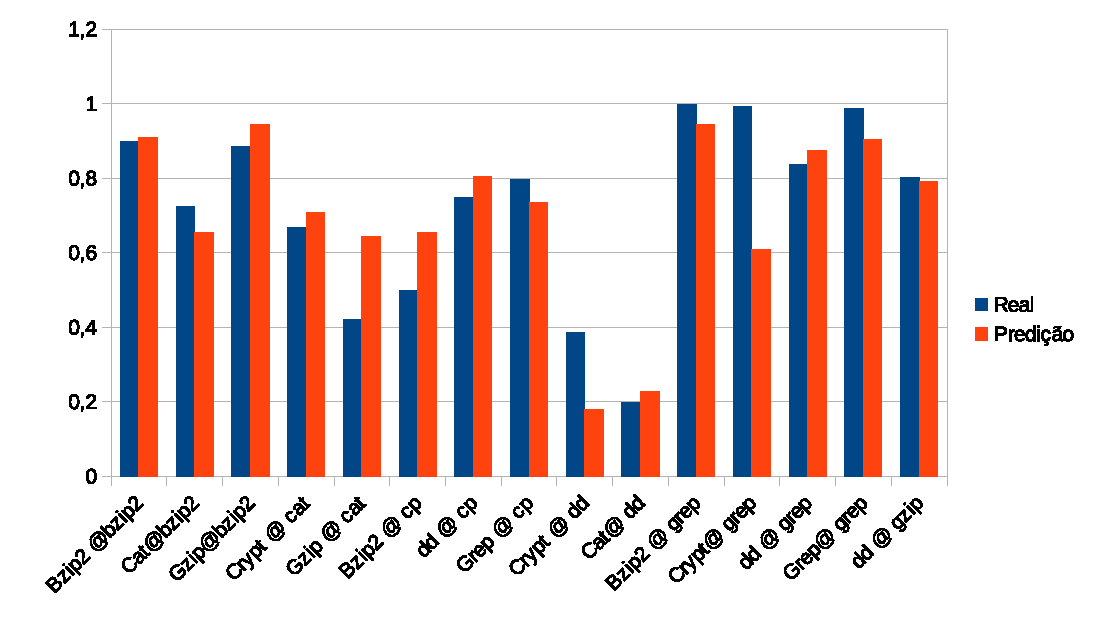
\includegraphics [keepaspectratio=true,scale=0.5]{graficos/linear.eps}
\caption{Comparativo entre a pontuação normalizada real e a pontuação predita utilizando regressão linear.}
\label{linear_predict}
\end{figure}   

A Figura \ref{linear_predict} apresenta os resultados da predição utilizando
regressão linear. Nota-se que em muitos casos os valores preditos pela
regressão linear possuem uma diferença maior para os valores reais do que na
predição feita por média ponderada. Assim, enquanto que Gzip @ Cat e bzip2 @ cp
obteve uma taxa de erro de 7,92\% e 1 ,65\% respectivamente na predição
utilizando média ponderada, na análise de regressão linear esse valores foram
de 53,6\% e 31,4\%. Mas ainda assim, para alguns casos, o modelo de regressão
linear conseguiu prever com uma taxa de erro mais baixa como por exemplo em dd
@ gzip e crypt @ cat, em que as taxas de erros da predição foram de 1,25\% e
5,67\% respectivamente.

Nos resultados apresentados na Figura \ref{poli_predict} percebe-se que dentre
os três modelos, a regressão polinomial é a que obtém valores de predição com
menores taxas de erro. Assim, enquanto que Crypt @ Grep obteve uma taxa de erro
de 41,5\% utilizando a média ponderada como modelo de predição, na análise de
regressão polinomial essa taxa de erro foi de 3,92\%. Dentre os resultados
apresentados na Figura \ref{poli_predict}, Cat @ dd foi o que obteve maior taxa
de erro, 19,5\%. 

\begin{figure}[!htb]
\centering
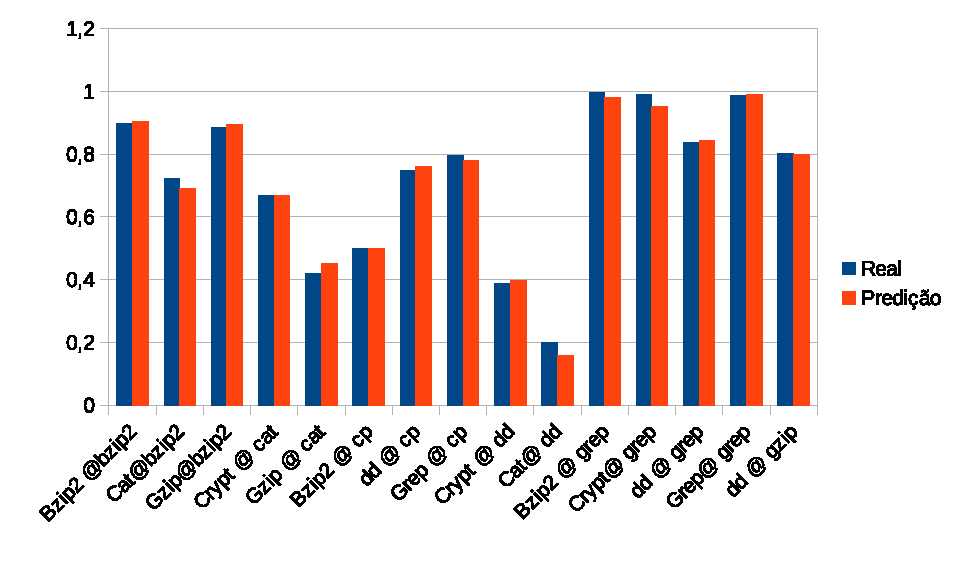
\includegraphics [keepaspectratio=true,scale=0.5]{graficos/poli.eps}
\caption{Comparativo entre a pontuação normalizada real e a pontuação predita utilizando regressão polinomial.}
\label{poli_predict}
\end{figure}  

A partir disso, a fim de verificar a qualidade dos modelos de regressão
aplicados, foi calculado o coeficiente de determinação R\textsuperscript{2}
tanto para a regressão linear quanto para a regressão polinomal. Dessa forma, a
regressão linear apresentou um coeficiente de determinação de 80,3\% enquanto
que a regressão polinomial atingiu um índice de 96,6\%, demonstrando que assim
como havia sido observado nos gráficos de predição, que a regressão polinomial
é o modelo mais adequado para a predição de desempenho dos dados se comparada
com a regressão linear.   

Como comparativo para os três modelos de predição foram calculados a média,
mediana e o maior erro de predição para todos os modelos. As Figuras
\ref{mean_error}, \ref{linear_error} e \ref{polinomial_error} apresenta esses
resultados.

\begin{figure}[!htb]
\centering
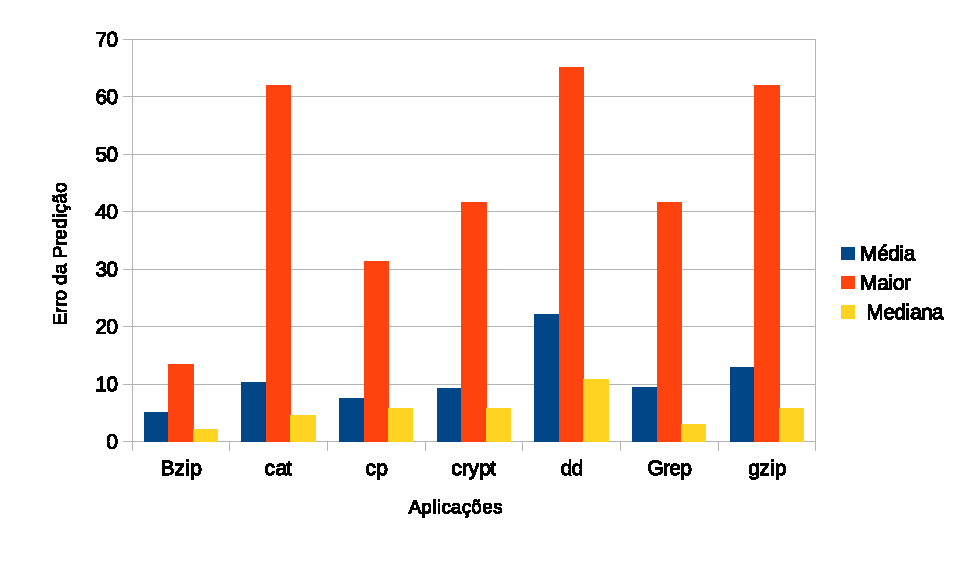
\includegraphics [keepaspectratio=true,scale=0.5]{graficos/mean_error.eps}
\caption{Média, mediana e erro máximo da predição de desempenho com o método da média ponderada}
\label{mean_error}
\end{figure}  

\begin{figure}[!htb]
\centering
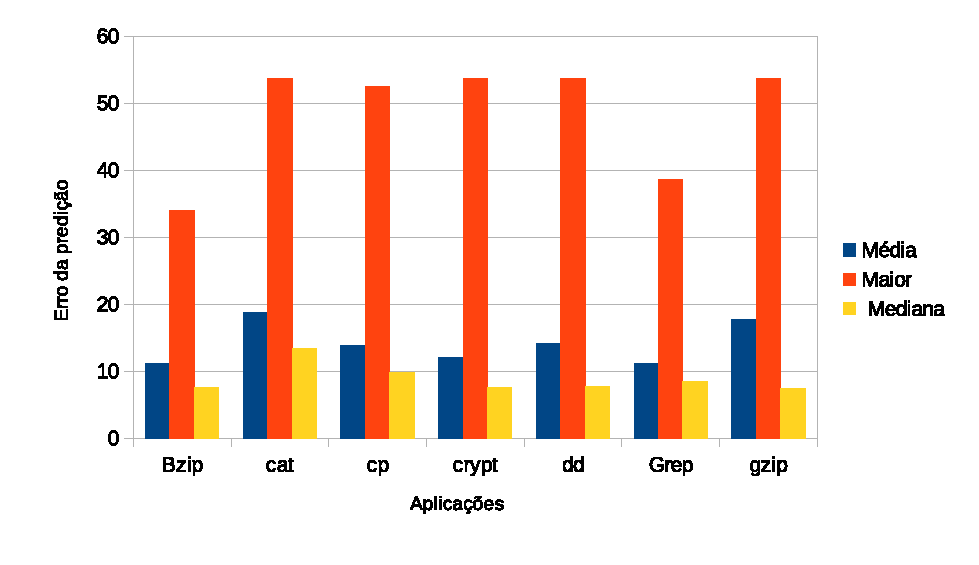
\includegraphics[width=.5\textwidth]{graficos/linear_error.eps}
\caption{Média, mediana e erro máximo da predição de desempenho com regressão linear}
\label{linear_error}
\end{figure}  

\begin{figure}[!htb]
\centering
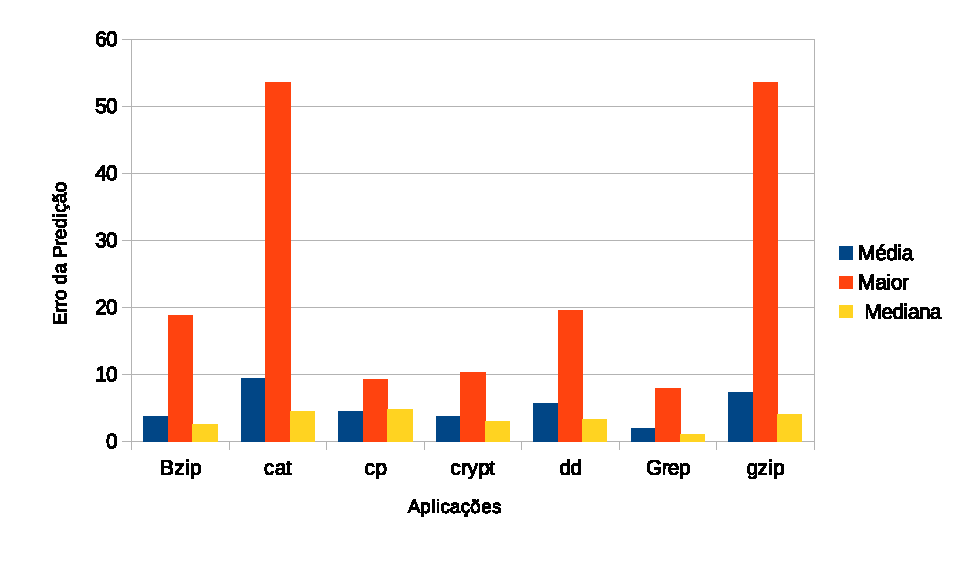
\includegraphics[width=.5\textwidth]{graficos/polinomial_error.eps}
\caption{Média, mediana e erro máximo da predição de desempenho com regressão polinomial}
\label{polinomial_error}
\end{figure}  


Assim como no trabalho de Koh \cite{koh2007}, comparada à média ponderada, a
regressão linear apresenta resultados inferiores relacionados a predição, com a
média de erros para todos os dados de 13,5\% e mediana de 8,8\%. Isso pode
estar relacionado ao fato da correlação entre as métricas de desempenho em
nível de sistema e a pontuação normalizada de uma aplicação não ser linear
\cite{koh2007}. Dessa forma, a regressão polinomial foi aplicada neste
trabalho. Além dos dados apresentados na Figura \ref{poli_predict} e no cálculo
do coeficiente de determinação R \textsuperscript{2}, os valores da média,
mediana e erro máximo apresentados na Figura \ref{polinomial_error} demonstram
que a regressão polinomial obtém resultados melhores para predição se comparada
com os modelos anteriores. Assim, de maneira geral, a média de erro para todos
os resultados alcançou um valor de 5\% e de mediana 2,7\%.


\section{Conclusão}
\label{sec:conclusao}

Nossos resultados demonstram que as tecnologias atuais de virtualização e de
computação em nuvem não garantem um isolamento efetivo entre máquinas virtuais
em um mesmo servidor físico. A tendência é que aplicações que possuem perfil
voltado para operações em disco interferem de maneira significativa no
desempenho outras aplicações  com o mesmo perfil, mesmo quando executadas em
máquinas virtuais diferentes. Aplicações com o perfil voltado para \textit{CPU}
interferem pouco contra aplicações com o perfil voltado para aplicações em
disco e vice-versa.

A partir dos dados coletados, aplicamos modelos estatísticos para a obteção da
predição de desempenho de uma aplicação a partir das métricas de desempenho em
nível de sistema. Assim como no trabalho de Koh \cite{koh2007}, a média
ponderada com o auxílio da análise por componente principal obteve resultados
melhores se comparada com a regressão linear. Dessa forma, aplicamos um modelo
regressão polinomial que apresentou ajustes mais aproximados para a predição de
desempenho de uma aplicação.

A avaliação da degradação de desempenho entre aplicações com o perfil voltado
para utilização de \textit{cpu} não foi realizada e pode ser considerada uma
limitação deste trabalho. De toda forma, entendemos que para as configurações
de \textit{hardware} do servidor utilizado neste estudo são necessárias um
número maior de máquinas virtuais executando \textit{benchmarking} de
\textit{cpu}, ao mesmo tempo, para que fosse possível observar algum tipo de
interferência e degradação em seus desempenhos.

Por fim, os procedimentos adotados neste trabalho promovem algumas
posssibilidades para trabalhos futuros, como estudo um comparativo entre os
diversos tipos de \textit{hypervisors} utilizados, levando-se em conta as
técnicas de virtualização paravirtualização e virtualização total, de modo que
se possa avaliar qual tipo de ferramenta, dada a técnica de virtualização,
trata melhor a interferência de desempenho entre as máquinas virtuais.

%------------------------------------------------------------------------------

\bibliographystyle{IEEEtran}
\bibliography{IEEEabrv,tcc-maxwell}

\end{document}
